\begin{figure}[htbp]
\centering
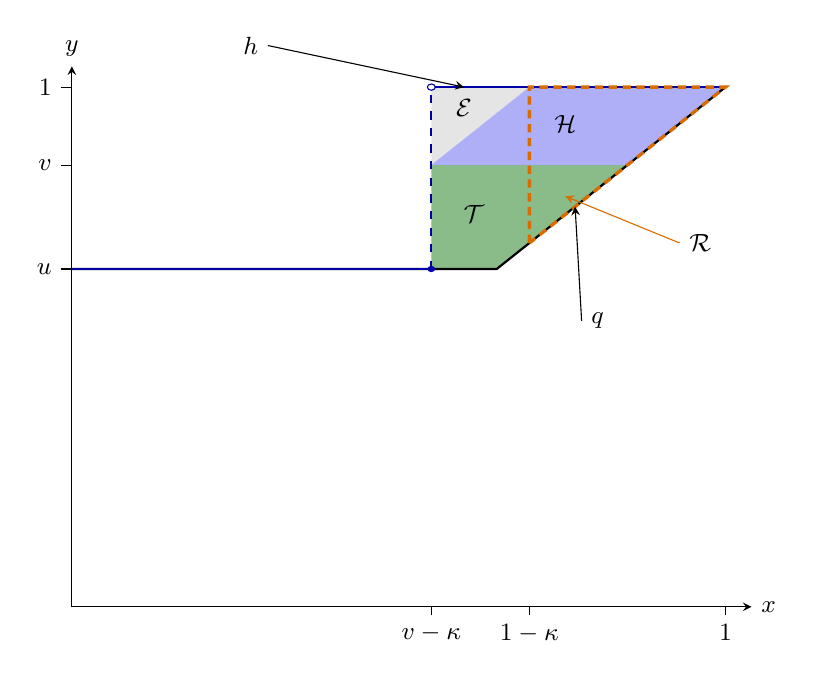
\begin{tikzpicture}[x=8.3cm,y=6.6cm,>=stealth,font=\small]
  \fill[black!10] (.55,.65)--(.55,1)--(1,1)--(.65,.65)--cycle;
  \fill[blue!40,opacity=.70] (.55,.85)--(.85,.85)--(1,1)--(.7,1)--cycle;
  \fill[green!50!black,opacity=.40] (.55,.65)--(.65,.65)--(.85,.85)--(.55,.85)--cycle;
  \draw[->] (0,0)--(1.04,0) node[right] {$x$};
  \draw[->] (0,0)--(0,1.04) node[above] {$y$};
  \draw[thick] (0,.65)--(.65,.65)--(1,1);
  \draw[thick,blue!65!black] (0,.65)--(.55,.65);
  \draw[thick,dashed,blue!65!black] (.55,.65)--(.55,1);
  \draw[thick,blue!65!black] (.55,1)--(1,1);
  \fill[blue!65!black] (.55,.65) circle[radius=.006];
  \filldraw[fill=white,draw=blue!65!black] (.55,1) circle[radius=.006];
  \draw[very thick,densely dashed,orange!85!black] (.7,.7)--(.7,1)--(1,1)--cycle;
  \draw (.55,0)--(.55,-.016) node[below] {$v-\kappa$};
  \draw (.7,0)--(.7,-.016) node[below] {$1-\kappa$};
  \draw (1,0)--(1,-.016) node[below] {$1$};
  \draw (0,.65)--(-.016,.65) node[left] {$u$};
  \draw (0,.85)--(-.016,.85) node[left] {$v$};
  \draw (0,1)--(-.016,1) node[left] {$1$};
  \node at (.615,.755) {$\mathcal T$};
  \node at (.755,.93) {$\mathcal H$};
  \node at (.6,.96) {$\mathcal E$};
  \draw[->,orange!85!black] (.93,.70) node[right,black] {$\mathcal R$} -- (.755,.79);
  \draw[->] (.3,1.08) node[left] {$h$} -- (.6,1);
  \draw[->] (.78,.55) node[right] {$q$} -- (.77,.77);
\end{tikzpicture}
\caption{An example with $\kappa=0.3$, $\ell=0.7$, and $u=0.65$.
The function $h$ equals $0.65$ at and before its jump at $0.55$ and equals $1$
after the jump. The dashed segment marks the jump, and the open and filled
points specify its value there. The
grey background together with the blue and green regions is $\mathcal E$.
The blue region is $\mathcal H$, and the green clipped triangle is
$\mathcal T$, where the infimum of the failure levels is
$v=0.85$. Region shading ignores boundary points. The orange outline marks
$\mathcal R$. In this example its
intersections with $\mathcal H$ and $\mathcal T$ partition $\mathcal R$
up to boundary points, so their combined area attains $\kappa^2/2$.}
\label{fig:excess-regions}
\end{figure}
